% !TEX TS-program = pdflatex
% !TEX encoding = UTF-8 Unicode

% This is a simple template for a LaTeX document using the "article" class.
% See "book", "report", "letter" for other types of document.

\documentclass[11pt]{article} % use larger type; default would be 10pt

\usepackage[utf8]{inputenc} % set input encoding (not needed with XeLaTeX)
\usepackage{graphicx}
\usepackage{subcaption}
\graphicspath{{./images/}}

%%% Examples of Article customizations
% These packages are optional, depending whether you want the features they provide.
% See the LaTeX Companion or other references for full information.

%%% PAGE DIMENSIONS
\usepackage{geometry} % to change the page dimensions
\geometry{a4paper} % or letterpaper (US) or a5paper or....
% \geometry{margin=2in} % for example, change the margins to 2 inches all round
% \geometry{landscape} % set up the page for landscape
%   read geometry.pdf for detailed page layout information

\usepackage{graphicx} % support the \includegraphics command and options

% \usepackage[parfill]{parskip} % Activate to begin paragraphs with an empty line rather than an indent

%%% PACKAGES
\usepackage{booktabs} % for much better looking tables
\usepackage{array} % for better arrays (eg matrices) in maths
\usepackage{paralist} % very flexible & customisable lists (eg. enumerate/itemize, etc.)
\usepackage{verbatim} % adds environment for commenting out blocks of text & for better verbatim
% These packages are all incorporated in the memoir class to one degree or another...
\usepackage{color}

%%% HEADERS & FOOTERS
\usepackage{fancyhdr} % This should be set AFTER setting up the page geometry
\pagestyle{fancy} % options: empty , plain , fancy
\renewcommand{\headrulewidth}{0pt} % customise the layout...
\lhead{}\chead{}\rhead{}
\lfoot{}\cfoot{\thepage}\rfoot{}

%%% SECTION TITLE APPEARANCE
\usepackage{sectsty}
\allsectionsfont{\sffamily\mdseries\upshape} % (See the fntguide.pdf for font help)
% (This matches ConTeXt defaults)

%%% ToC (table of contents) APPEARANCE
\usepackage[nottoc,notlof,notlot]{tocbibind} % Put the bibliography in the ToC
\usepackage[titles,subfigure]{tocloft} % Alter the style of the Table of Contents
\renewcommand{\cftsecfont}{\rmfamily\mdseries\upshape}
\renewcommand{\cftsecpagefont}{\rmfamily\mdseries\upshape} % No bold!

%%% END Article customizations

%%% The "real" document content comes below...

\title{Design and Evaluation of a Machine Vision System for Identifying Cracked PV Panels}
\author{Jerome Wynne}
%\date{} % Activate to display a given date or no date (if empty),
         % otherwise the current date is printed 

\begin{document}
\maketitle

\section{Problem Description}

This work developed a system for automatically identifying cracks in PV panels from their 2D grayscale computed tomography images. 50 images were provided. 38 of these were deemed to be cracked. Several of these images are shown in Figure \ref{fig:sample_panels}.
\begin{figure}[h!]
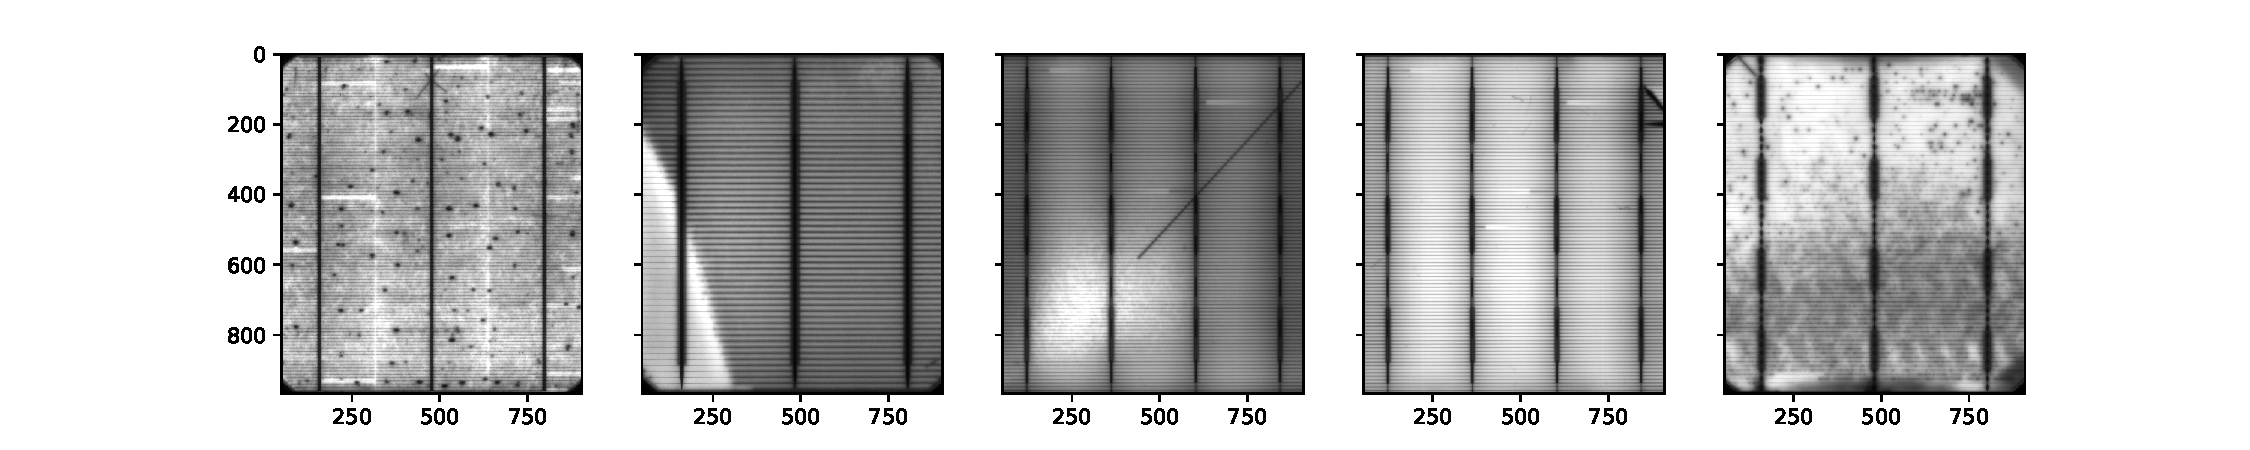
\includegraphics[width=\textwidth]{sample_panels.pdf}
\caption{Scans of the PV panels that were analyzed for damage. The first, third, fourth, and fifth panels from the left contain cracks. Pock-marks similar to those seen on the first panel were not regarded as cracks.}
\label{fig:sample_panels}
\end{figure}

 The median frame height for these images was 965 pixels; their width was similar. Depending on the model and filters used, the images were shrunk for processing.

As can be deduced from Figure \ref{fig:crack_v_scratch}, it was sometimes difficult to ascertain whether a given mark was a crack or a scratch. For the purposes of this work, the latter were considered to be fainter and wigglier - heuristic measures in the absence of any conveniently quantifiable differences. The labels themselves consisted of manually drawn binary masks. Each pixel in a mask was in effect an indicator representing whether the associated image pixel was part of a crack. {\color{red}The masks created were validated by a panel inspector}. The centers of thick cracks were not labelled, on the basis that they would make learning difficult if small kernel sizes were to be used. For example, a 20$\times$20 window centered on a thick crack would be a dark array almost indistinguishable from other dark non-crack regions in the images (in the absence of positional information, at least).

\begin{figure}[h!]
\centering
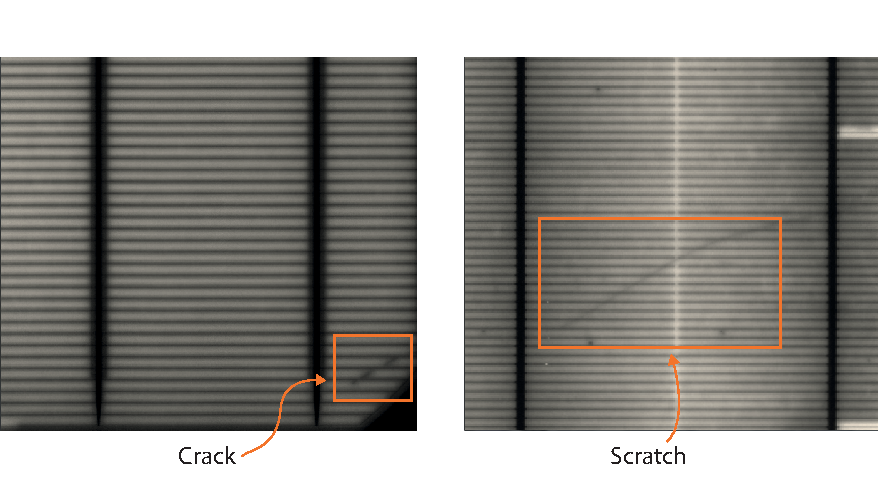
\includegraphics[width=0.7\textwidth]{crack_v_scratch.pdf}
\caption{Distinguishing between cracks and scratches was difficult in certain cases, making ground truth labels somewhat subjective.}
\label{fig:crack_v_scratch}
\end{figure}

Observed sources of noise in the images were as follows:
\begin{itemize}
	\item Dead cells (cells that were unusually bright relative to their neighbors)
	\item Scratches and marks (dark lines)
	\item Debris in the scanner (dark patches)
	\item Hail damage (dark pock-marks)
	\item Variation in the panel model (variation in the panel's layout)
	\item Delamination (low-frequency intensity variation)
\end{itemize}

\begin{figure}[h!]
\centering
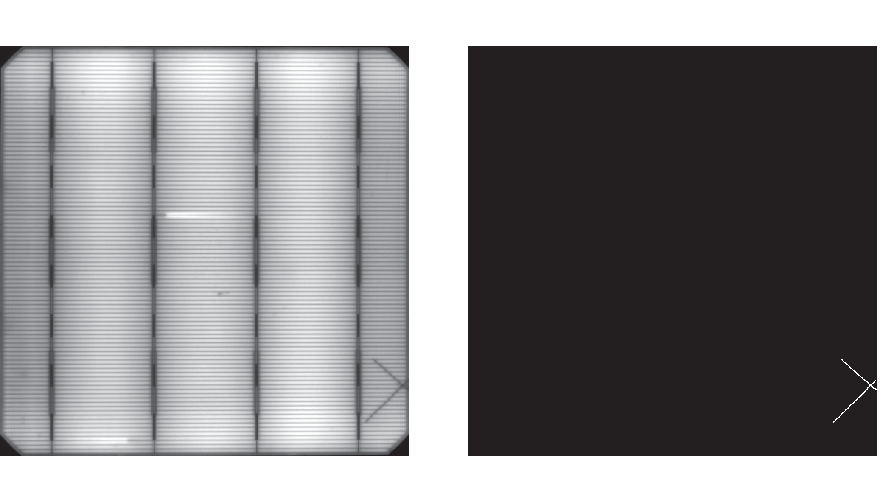
\includegraphics[width=0.7\textwidth]{mask_example.pdf}
\caption{An image of a panel and its associated set of labels.}
\label{fig:mask_example}
\end{figure}

The ideal panel classifier was defined as being one that:
\begin{itemize}
	\item Provided accurate classification of panels according to the classes cracked/not cracked.
	\item Provided estimates of class membership probabilities to allow operators to tune the model's sensitivity.
	\item Provided per-pixel classification to enable an operator to quickly the area flagged as being cracked.
	\item Operated within reasonable time and compute constraints.
\end{itemize}
Interpretability was not considered a priority.


\subsection{Pre-Processing}
Various filters were applied to the images in an attempt to emphasize cracks and suppress other features. Horizontal differencing of pixel intensities proved to be an effective means of filtering the horizontal cells. A $3\times3$ Laplace filter was used to achieve this effect - a Prewitt filter was also tested, but yielded basically identical results.  A large proportion of the cracks were found to propagate diagonally, an attribute that was exploited by applying a pair of Gabor filters to the image then taking the magnitude of the difference between their real components. The Gabor kernel used is shown in Figure \ref{fig:Gabor_kernel}. By combining horizontal differencing and the described Gabor filtering, the diagonal cracks were substantially enhanced relative to the rest of the image, with the exception of the panel's corners. This process and its results are shown in \ref{fig:filter_process}.

\begin{figure}
\centering
\includegraphics[width = 0.5\textwidth]{Gabor_kernel.pdf}
\caption{The real component of the two Gabor filters applied to the images. The other filter was equivalent but flipped across the vertical axis.}
\label{fig:Gabor_kernel}
\end{figure}

As an alternative method for extracting information pertaining to edge orientation, histograms of oriented gradients were used. An image's gradients were estimated using a combination of Laplace filters, then their magnitudes were accumulated in bins corresponding to distinct orientations. The bin counts in each cell were normalized relative to neighboring cells, then the cell histograms were flattened and concatenated to be fed into classifiers that accepted vector inputs. So far, HOGs have only been tested against classifiers accepting vectors: one possible line of enquiry is to pass them to classifiers accepting tensors of higher orders. Aside from HOGs, the Hough transform may also be a promising candidate for identifying diagonal lines that do not correspond to the panel's corners. It has yet to be trialled.


\subsection{Modeling}
The models trialled so far include:
\begin{itemize}
	\item Generative models against pixel intensity (i.e. modeling local pixel intensities using a multivariate normal distribution)
	\begin{itemize}
		\item These were also tested as filters, the output of which was fed to a nonlinear classifier. An example of this sequence is shown in Figure \ref{fig:normal_then_randomforest}.
	\end{itemize}
	\item Canned classifiers from \texttt{sklearn} - random forest, radial-basis function support vector machines, logistic regression.
	\item Shallow convolutional neural networks against pixel intensity.
\end{itemize}

\begin{figure}[h!]
\includegraphics[width=\textwidth]{normal_then_randomforest.pdf}
\caption{Left: raw image. Center: Log-odds returned by a normal model fit to 20$\times$20 patches of cracks. Right: Crack probabilities returned by a random forest fit to the log-odds returned by the normal model. (This needs a colorbar!)}
\label{fig:normal_then_randomforest}
\end{figure} 

TBC

\begin{figure}
\centering
  	 \begin{subfigure}[b]{1\textwidth}
   	\includegraphics[width=\textwidth]{demo_images.pdf}
   	\caption{Raw images.}
   	\label{fig:a} 
	\end{subfigure}

  	 \begin{subfigure}[b]{1\textwidth}
   	\includegraphics[width=\textwidth]{sobelv.pdf}
   	\caption{Vertical Sobel filter.}
   	\label{fig:b} 
	\end{subfigure}
	
  	 \begin{subfigure}[b]{1\textwidth}
   	\includegraphics[width=\textwidth]{sobelv_gaborne.pdf}
   	\caption{Vertical Sobel filtering followed by a Gabor filter.}
   	\label{fig:d} 
	\end{subfigure}
	
  	 \begin{subfigure}[b]{1\textwidth}
   	\includegraphics[width=\textwidth]{sobelv_gabordiff.pdf}
   	\caption{Vertical Sobel filtering followed by a difference of two Gabor-filtered images.}
   	\label{fig:f} 
	\end{subfigure}
	
	\begin{subfigure}[b]{1\textwidth}
   	\includegraphics[width=\textwidth]{demo_masks.pdf}
   	\caption{Original image masks (i.e. ground truth).}
   	\label{fig:f} 
	\end{subfigure}
\caption{}
\end{figure}


\newpage
\section*{Placement Update}
\subsection*{Last time we met}
\begin{itemize}
	\item 3rd July (2 weeks ago)
	\item I presented:
	\begin{itemize}
		\item The labelling strategy I have been using (i.e. per-pixel binary masks).
		\item An image subsetting and augmentation procedure.
		\item Canned classifiers against raw pixel intensities.
		\item Canned classifiers against vectorized data of the prominence of intensity gradients in certain directions (i.e. Histograms of oriented gradients).
		\item A proposed scheme for making adjacent pixel labels more consistent with one another (more on this later).
		\item Problems w.r.t. splitting the data and obtaining robust classification accuracy estimates (i.e. the dataset is small).
	\end{itemize}
	\item We agreed I should expand the feature space, \emph{by any means necessary}.
\end{itemize}

\subsection*{What I've been up to since then}
\begin{itemize}
	\item Spent a fantastic couple of weeks in Barbados.
	\begin{figure}[h!]
		\centering
		\includegraphics[width=0.7\textwidth]{maldives.png}
		\caption{My co-working space.}
	\end{figure}
	\item Time split: 25\% creating new image representations, 30\% reading about modelling strategies, 10\% building models, 35\% building testing infrastructure.
	\item Other image representations:
		\begin{itemize}
			\item Gabor filters and other edge/ridge-based filters.
			\item Global fourier transform.
			\item Local fourier transform.
			\item Hough transform.
			\item Local binary patterns (more on these later).
			\item Hierarchical filtering (\emph{a la} convnets).
		\end{itemize}
	\item Modelling strategies: relaxation labelling and Markov random fields.
		\begin{itemize}
			\item Description image.
			\item Performance depends on having an initial classifier that is - at minimum - passable (obviously).
			\item Yields an accuracy increase of several per cent.
			\item Disagreement regarding choice of compatibility function and update equations (former: transition probabilities, correlations, mutual information).
			\item Markov random field model:  might be more appropriate/effective?
		\end{itemize}
	\item Model implementation: simple convolutional neural network.
		\begin{itemize}
			\item Initial performance suggests an accuracy of c. 85\% against a balanced set of 20x20 image patches.
			\item Against genuine images, where approx. < 0.1\% of patches correspond to cracks, this translates into poorer performance.
			\item Plan to experiment with:
			\begin{itemize}
				\item Other patch sizes.
				\item Increasing the number of input channels (e.g. filtered version of the patch, rescaling the entire image down to the patch's size, providing a map marking the patch's position within the image and so on).
				\item Using spatial transformer networks (learning a transformation mapping the input to a `'canonical'' (i.e. standardized) representation of a crack) to improve classification accuracy and act as an attention mechanism (to reduce the fraction of an input image that needs to be processed).
				\item Making the network deeper (it's only two layers at the moment).
				\item Implementing filters mid-network (e.g. applying a Hough transform to the network's output, then feeding that into a multilayer perceptron).
			\end{itemize}
		\end{itemize}
	\item Model implementation: Gaussian discriminant analyzer.
	\begin{itemize}
		\item Need to make it compatible with the testing API.
		\item It seemed to do okay - needs to be plugged into the new testing framework.
		\begin{figure}[t!]
			\centering
			\begin{subfigure}[b]{0.6\textwidth}
				\includegraphics[width=\textwidth]{gaussian_discriminant_analysis_means.png}
				\caption{Group means ($20 \times 20$ patch).}
   				\label{fig:a} 
			\end{subfigure}
			\begin{subfigure}[b]{0.6\textwidth}
				\includegraphics[width=\textwidth]{gaussian_discriminant_analysis_variances.png}
				\caption{Diagonal entries of group covariance matrices.}
   				\label{fig:b} 
			\end{subfigure}
		\end{figure}
		\begin{figure}[t!]
		\centering
		\begin{subfigure}[t]{0.3\textwidth}
			\includegraphics[width=\textwidth]{unfiltered_input_to_GDA.png}
			\caption{Query image.}
   			\label{fig:c} 
		\end{subfigure}
		\begin{subfigure}[t]{0.3\textwidth}
			\includegraphics[width=\textwidth]{GDA_unfiltered_log_odds.png}
			\caption{Log-odds of query image.}
   			\label{fig:d} 
		\end{subfigure}
		\end{figure}
	\item Testing infrastructure:
		\begin{itemize}
			\item All in TensorFlow.
			\item Separates preprocessing and modelling.
			\item Provides a consistent modelling environment, making it easier to form ensembles or chain models later.
			\item Standardizes performance reporting and allows models to be visualized (court oisie de TensorBoard).
			\item Easily extensible to larger datasets.
			\item Ensures the data splitting procedure is transparent and consistent.
			\item Demo.
			\begin{figure}
			\centering
				\includegraphics[width=0.7\textwidth]{tboard_demo_graph.png}
				\caption{Graph of the convolutional network that has been implemented, courtesy of TensorBoard.}
			\end{figure}
			\begin{figure}
				\includegraphics[width=\textwidth]{tboard_demo_plot.png}
				\caption{Using TensorBoard we can create standardized reports, which should make evaluating models more straightforward.}
			\end{figure}
			\begin{figure}
				\includegraphics[width=\textwidth]{tboard_demo_images.png}
				\caption{A sample of the filters learnt by the first layer. These may be useful for preprocessing images for other classifiers.}
			\end{figure}
		\end{itemize}
	\end{itemize}
\end{itemize}

\begin{figure}
	\includegraphics[width=\textwidth]{relaxation-labelling.pdf}
\end{figure}

\subsection*{Problems I have and what I plan to do about them}
\begin{itemize}
	\item Data:
	\begin{itemize}
		\item Splitting the dataset after sampling patches from the images results in isomorphic training and validation datasets: The dataset must be split at the full-image level for our performance measures to be valid.
		\item Because the dataset is so small, the splitting is very granular. Limited representation of rare crack types in the data available means that the validation and training datasets contain different distributions of crack types.
		\item Consequently,  model fit and accuracy metrics are both very sensitive to the split chosen. If the training data contains all rare cracks, the accuracy will appear high. If it contains unusual cracks, a model will appear to perform badly.
		\item If this problem afflicts all models equally, then comparisons of performance between models are valid. If not, then we cross-validation is necessary. This is time-consuming; additionally, comparing models becomes more subjective.
		\item If you have Azure access, please could I have a copy of the additional data?
	\end{itemize}
	\item Middle of placement:
	\begin{itemize}
		\item Wary of reaching week 8 with lots of half-finished, half-evaluated models.
		\item Intend to focus on:
		\begin{itemize}
			\item Convolutional neural networks
			\item Markov random fields.
		\end{itemize}
		\item Current objective: solve the PV panel crack identification problem, write a report summarizing the methods applied and their efficacy..
	\end{itemize}
	\item Feedback:
	\begin{itemize}
		\item Pointers/warnings?
		\item Suggestions for making sure I produce something fruitful? (What would \emph{you} find useful for me to deliver at the end of this placement? Report, model, code?)
		\item Witticisms?
		\item Presenting style / communication skills?
	\end{itemize}
\end{itemize}

\end{document}
